% This is "sig-alternate.tex" V2.1 April 2013
% This file should be compiled with V2.5 of "sig-alternate.cls" May 2012
%
% This example file demonstrates the use of the 'sig-alternate.cls'
% V2.5 LaTeX2e document class file. It is for those submitting
% articles to ACM Conference Proceedings WHO DO NOT WISH TO
% STRICTLY ADHERE TO THE SIGS (PUBS-BOARD-ENDORSED) STYLE.
% The 'sig-alternate.cls' file will produce a similar-looking,
% albeit, 'tighter' paper resulting in, invariably, fewer pages.
%
% ----------------------------------------------------------------------------------------------------------------
% This .tex file (and associated .cls V2.5) produces:
%       1) The Permission Statement
%       2) The Conference (location) Info information
%       3) The Copyright Line with ACM data
%       4) NO page numbers
%
% as against the acm_proc_article-sp.cls file which
% DOES NOT produce 1) thru' 3) above.
%
% Using 'sig-alternate.cls' you have control, however, from within
% the source .tex file, over both the CopyrightYear
% (defaulted to 200X) and the ACM Copyright Data
% (defaulted to X-XXXXX-XX-X/XX/XX).
% e.g.
% \CopyrightYear{2007} will cause 2007 to appear in the copyright line.
% \crdata{0-12345-67-8/90/12} will cause 0-12345-67-8/90/12 to appear in the copyright line.
%
% ---------------------------------------------------------------------------------------------------------------
% This .tex source is an example which *does* use
% the .bib file (from which the .bbl file % is produced).
% REMEMBER HOWEVER: After having produced the .bbl file,
% and prior to final submission, you *NEED* to 'insert'
% your .bbl file into your source .tex file so as to provide
% ONE 'self-contained' source file.
%
% ================= IF YOU HAVE QUESTIONS =======================
% Questions regarding the SIGS styles, SIGS policies and
% procedures, Conferences etc. should be sent to
% Adrienne Griscti (griscti@acm.org)
%
% Technical questions _only_ to
% Gerald Murray (murray@hq.acm.org)
% ===============================================================
%
% For tracking purposes - this is V2.0 - May 2012

\documentclass{sig-alternate-05-2015}
\usepackage{epstopdf}
\usepackage{cite}
\usepackage{floatrow,graphics,subfig}
\usepackage[square, comma, sort&compress, numbers]{natbib}
\usepackage{hyperref}
\usepackage{pifont, footnote}
%\usepackage[pdfpagelabels,hypertexnames=false,breaklinks=true,bookmarksopen=true,bookmarksopenlevel=2]{hyperref}



\begin{document}
\bibliographystyle{unsrt}
% Copyright
\setcopyright{acmcopyright}
%\setcopyright{acmlicensed}
%\setcopyright{rightsretained}
%\setcopyright{usgov}
%\setcopyright{usgovmixed}
%\setcopyright{cagov}
%\setcopyright{cagovmixed}


% DOI
\doi{10.475/123_4}

% ISBN
\isbn{123-4567-24-567/08/06}

%Conference
\conferenceinfo{PLDI '13}{June 16--19, 2013, Seattle, WA, USA}

\acmPrice{\$15.00}

%
% --- Author Metadata here ---
\conferenceinfo{WOODSTOCK}{'97 El Paso, Texas USA}
%\CopyrightYear{2007} % Allows default copyright year (20XX) to be over-ridden - IF NEED BE.
%\crdata{0-12345-67-8/90/01}  % Allows default copyright data (0-89791-88-6/97/05) to be over-ridden - IF NEED BE.
% --- End of Author Metadata ---

\title{DRET: A System for Detecting Evil-twin Attacks in Smart Homes%\titlenote{(Produces the permission block, and
%copyright information). For use with
%SIG-ALTERNATE.CLS. Supported by ACM.}
}
\subtitle{
%\titlenote{A full version of this paper is available as
%\textit{Author's Guide to Preparing ACM SIG Proceedings Using
%\LaTeX$2_\epsilon$\ and BibTeX} at
%\texttt{www.acm.org/eaddress.htm}}
}
%
% You need the command \numberofauthors to handle the 'placement
% and alignment' of the authors beneath the title.
%
% For aesthetic reasons, we recommend 'three authors at a time'
% i.e. three 'name/affiliation blocks' be placed beneath the title.
%
% NOTE: You are NOT restricted in how many 'rows' of
% "name/affiliations" may appear. We just ask that you restrict
% the number of 'columns' to three.
%
% Because of the available 'opening page real-estate'
% we ask you to refrain from putting more than six authors
% (two rows with three columns) beneath the article title.
% More than six makes the first-page appear very cluttered indeed.
%
% Use the \alignauthor commands to handle the names
% and affiliations for an 'aesthetic maximum' of six authors.
% Add names, affiliations, addresses for
% the seventh etc. author(s) as the argument for the
% \additionalauthors command.
% These 'additional authors' will be output/set for you
% without further effort on your part as the last section in
% the body of your article BEFORE References or any Appendices.

%\numberofauthors{8} %  in this sample file, there are a *total*
% of EIGHT authors. SIX appear on the 'first-page' (for formatting
% reasons) and the remaining two appear in the \additionalauthors section.
%
\author{
% You can go ahead and credit any number of authors here,
% e.g. one 'row of three' or two rows (consisting of one row of three
% and a second row of one, two or three).
%
% The command \alignauthor (no curly braces needed) should
% precede each author name, affiliation/snail-mail address and
% e-mail address. Additionally, tag each line of
% affiliation/address with \affaddr, and tag the
% e-mail address with \email.
%
% 1st. author
%\alignauthor
\affaddr{Zhanyong Tang$^\dag$, Yujie Zhao$^\dag$, Lei Yang$^\dag$, Shengde Qi$^\dag$, Dingyi Fang$^\dag$\thanks{Correspondence should be addressed to Dingyi Fang, Email: dyf@nwu.edu.cn}}\\
\affaddr{Xiaojiang Chen$^\dag$, Xiaoqing Gong$^\dag$, Zheng Wang$^\ddag$}\\
\affaddr{$^\dag$School of Information Science and Technology, Northwest University, Xi'an, 710127, P.R. China.}\\
\affaddr{$^\ddag$School of Computing and Communications, Lancaster University, UK.}\\
}

      %\affaddr{P.O. Box 5000}\\
       %\email{lleipuner@researchlabs.org}


% There's nothing stopping you putting the seventh, eighth, etc.
% author on the opening page (as the 'third row') but we ask,
% for aesthetic reasons that you place these 'additional authors'
% in the \additional authors block, viz.
%\additionalauthors{Additional authors: John Smith (The Th{\o}rv{\"a}ld Group,
%email: {\texttt{jsmith@affiliation.org}}) and Julius P.~Kumquat
%(The Kumquat Consortium, email: {\texttt{jpkumquat@consortium.net}}).}
%\date{30 July 1999}
% Just remember to make sure that the TOTAL number of authors
% is the number that will appear on the first page PLUS the
% number that will appear in the \additionalauthors section.
\maketitle

\begin{abstract}

Evil-twin is one of most commonly attacks in the WIFI environments, with which an attacker can steal sensitive information by cloning a fake AP in Smart Homes. The current approaches of detecting Evil-twin AP uses some identities/fingerprints of legitimated APs to identify rouge APs. Prior work in the area uses information like SSIDs, MAC addresses, and network traffics to detect bogus APs. However, such information can be easily intimated by the attacker, leading to low detection rates.

This paper introduces a novel Evil-Twin AP detection method based on received signal strength indicator (RSSI). Our approach exploits the fact that the AP location is relatively stable in Smart Homes, which is to great extent to meet the requirement of the detection factor not easy to imitate as previous refer. We employ two detection strategies: a single position detection and a multi-positioned detection methods. Our approach exploits the multipath effect of WIFI signals to translate the problem of attack detection into AP positioning detection. Compared to classical detection methods, our approach can perform detection without relying on professional devices. Experimental results show that the single position detection approach achieves 20 seconds' reduction of delay time with an accuracy of 98\%, whereas the multi-positioned detection approach achieves 90\% correct.

%Evil-Twin is one of most commonly attack in the WIFI environment. Attackers can implement an Evil-Twin Attack by cloning an rouge AP to steal private information, open door secret, bank account password, etc in Smart Home. Current Evil-Twin AP detection depend on comparing some identities/fingerprints of rouge AP to those of legitimated APs. Past proposals for addressing the differences between rouge APs and legitimated APs rely on SSID, MAC, network traffic, etc, but all of them can easily be intimated by attacker leading to the detection rate decreased.
%
%This paper introduces an Evil-Twin AP detection based on RSSI in Smart Home, which depends on the fact that the location of APs are relatively stable in the scenarios of Smart Home. It is consisted by two detection strategies: single position detection and multiple position cooperative detection. This method utilizing multipath effect, convert Attack Detection into Positioning. Compared to traditional detection methods, the proposed method could complete detection process without professional devices. Experimental results showed that single position detection reduced delay time to 20s and raised accuracy to 98\%, and the multiple position detection raised accuracy to 90\%.


\end{abstract}


%
% The code below should be generated by the tool at
% http://dl.acm.org/ccs.cfm
% Please copy and paste the code instead of the example below.
%
%\begin{CCSXML}
%<ccs2012>
% <concept>
%  <concept_id>10010520.10010553.10010562</concept_id>
%  <concept_desc>Computer systems organization~Embedded systems</concept_desc>
%  <concept_significance>500</concept_significance>
% </concept>
% <concept>
%  <concept_id>10010520.10010575.10010755</concept_id>
%  <concept_desc>Computer systems organization~Redundancy</concept_desc>
%  <concept_significance>300</concept_significance>
% </concept>
% <concept>
%  <concept_id>10010520.10010553.10010554</concept_id>
%  <concept_desc>Computer systems organization~Robotics</concept_desc>
%  <concept_significance>100</concept_significance>
% </concept>
% <concept>
%  <concept_id>10003033.10003083.10003095</concept_id>
%  <concept_desc>Networks~Network reliability</concept_desc>
%  <concept_significance>100</concept_significance>
% </concept>
%</ccs2012>
%\end{CCSXML}

%\ccsdesc[500]{Computer systems organization~Embedded systems}
%\ccsdesc[300]{Computer systems organization~Redundancy}
%\ccsdesc{Computer systems organization~Robotics}
%\ccsdesc[100]{Networks~Network reliability}


%
% End generated code
%

%
%  Use this command to print the description
%
\printccsdesc

% We no longer use \terms command
%\terms{Theory}

\keywords{Smart Homes; Evil-Twin Attack; RSSI; Detection}

\section{INTRODUCTION}
Have you image that one day someone would open your intelligent door when you are outside, turn on gas valve when you are sleeping and stealing your bank count when you are surfing on the Internet? After the traditional internet and intelligent transportation internet, the attacker can put his claws to the Smart Homes Internet\cite{Chan200855},It is not an exaggeration to say that these attacks are invading every corner of our lives with the rapid development of wireless communication technology, such as WIFI, 4G, GPS etc\cite{184004,6566953}.One of the most commonly attacks in the WIFI environment is referred to as the Evil Twin Attack which occurs when an adversary clones an AP with the same identity (or SSID) as an authentic AP.The bogus AP then exploits automatic access point selection techniques to trick a wireless client to connect to itself. Such fake APs are also known as Evil-Twin AP (Rouge AP or Fake AP)\cite{1495975}.An adversary can use an Evil-Twin AP as a platform to launch a variety of attacks, such as privacy and data thelf. It is easily for the rogue AP to obtain information from the WIFI environment to compromise the security of the user. Smart Homes that rely on WIFI are also indispensable for suffering from Evil Twin Attacks. For instance, the Evil-Twin AP can hijack the DNS protocol and redirect the clients to a malicious server to steal the password of fingerprint lock or turning on the gas valve.

Because of the serious consequence, Evil-Twin AP detection has recently received much attention\cite{978156,7157983}.There are two widely used approaches in this domain. One is extracting unique traffic characteristics from the network flow\cite{Bratus,2006,fingerprinting,6258210}. For example, to distinguish authorized WLAN hosts from unauthorized WLAN hosts connected to rogue access points by analyzing traffic characteristics, such as packet arrival time, request/response time of continuous ACK in TCP traffic. These methods are affected by the network's type, bandwidth and congestion. Purely relying on network traffics can result in poor detection performance because the detection algorithms can miss some rouge APs with high imperceptibility. The other approach, namely fingerprint identification detection methods, uses hard-ware features\cite{1378413,Wei,POR,6007016,Mano,682342},to different the rogue APs from authentic APs. This is achieved by collecting key information of the authentic APs, such as firmware, chip, driver etc. Such an approach relies on the assumption that it is difficult for the attacker to build an AP with identical hardware information. However, building a fingerprint library is non-trivial. Moreover, extracting the fingerprints takes a long time, making such approaches infeasible when real-time is an essential requirement. Broadly speaking, the essence of Evil Twin detection is to find the as many differences between the rouge AP and the authentic AP as possible.

This paper introduces a novel method for detecting Evil-Twin APs, Our approach is based on the received signal strength indicator (RSSI). Our approach targets Smart Homes and exploits the fact the position of an AP is often fixed in a Smart Home environment. The main benefit of RSSI measurement based systems is that they do not require any additional sensor/actuator infrastructure but use already available communication parameters. By using RSSI, we can estimate the distance between the signal point and the receiving point \cite{levisrssi,Kotz,1212671,Kotaru,6195606,Rai,Liu,Sen,Schulz}.The work we are presenting relies only on received signal strength measurements from wireless radio access points to determine their possible position. In Smart Homes, The position of each AP is fixed and the RSSI signal is relatively stable, which is to great extent to meet the requirements of the detection factor not easy to imitate as previous refer. The challenge however is to identify the rouge APs in the case of that the intensity of the rouge AP is greater than that of the authentic AP. According to the 802.11 standard, when there are multiple APs existing nearby, a WLAN client will always choose the AP with the strongest signal to connect to\cite{6007016,4367937,McCoy}.

Unlike past approaches, our detection factor is not easily to imitate as the the AP's position is stable in smart homes. Hence, in some cases, those APs who are not at pre-determined position may have been forged. Our experimental results show that the proposed approach can effectively identify rouge APs. Our approach achieves on average a successful rate of 96\% with less than 20s testing delay.

The main contributions of this paper are, (1) It is first the Evil-Twin attack detection system for Smart Homes, (2) It is also the first to demonstrate RSSI can be used as a means for detecting Evil-Twin Attacks in smart homes. Although our approach assumes the location of the AP is stable, the essential idea can be expanded to the other WIFI environments.
\section{BACKGROUD}
SSID and BSSID is always used to identify WIFI hot point since the protocol 802.11 does not define a strong sign to do it. In fact, both of them could be easily got by attacker, because the wireless network not only share the media but also cannot control the signal range. Although the access point is protected by password and sophisticated encryption, for an experienced attacker, it is not difficult to crack it during a short time. Once the attacker got the password, they will soon forge a same one called Evil-Twin AP (Rouge AP or Fake AP), is not easier recognized by user. Over the past few years, this kind of attack mainly exists in some public environments such as airports and cafes. However, as the development of the IoT, the attack value of private WIFI rises rapidly, and the attack develops towards the private WIFI in the Smart Home and other environments. Once the user connects the network to the Fake AP, the intruder can control the network environment of the user, and further, privacy sniffing, malicious data tampering and others advanced attack can be realized. The behavior of the intelligent device even can be controlled, for instance, opening or closing an intelligent lock, etc.

According to IEEE 802.11, when there is lots of APs around with the terminal, one with the strongest signal to be connected\cite{6007016}. So the Fake AP is always be put at the nearest of attack target in order to be choose. This kind of attack can be called Fishing, which contains active Fishing and passive Fishing. Passive Fishing is namely that the Fake AP is just waiting for the connection from the terminal. This kind of attack cannot easily be found since it does not affect the Real AP, at the same time, the attack success rate is not high. Active Fishing means that to connect with the terminal, Fake AP cut of the connection between Real AP and the terminal by Evil-Twin Attack. Such attack can be carried out to precise attacks without affecting the other equipment except the target.

\section{ATTACK SCENARIO AND ASSUMPTIONS}
\begin{figure}[h]
\centering
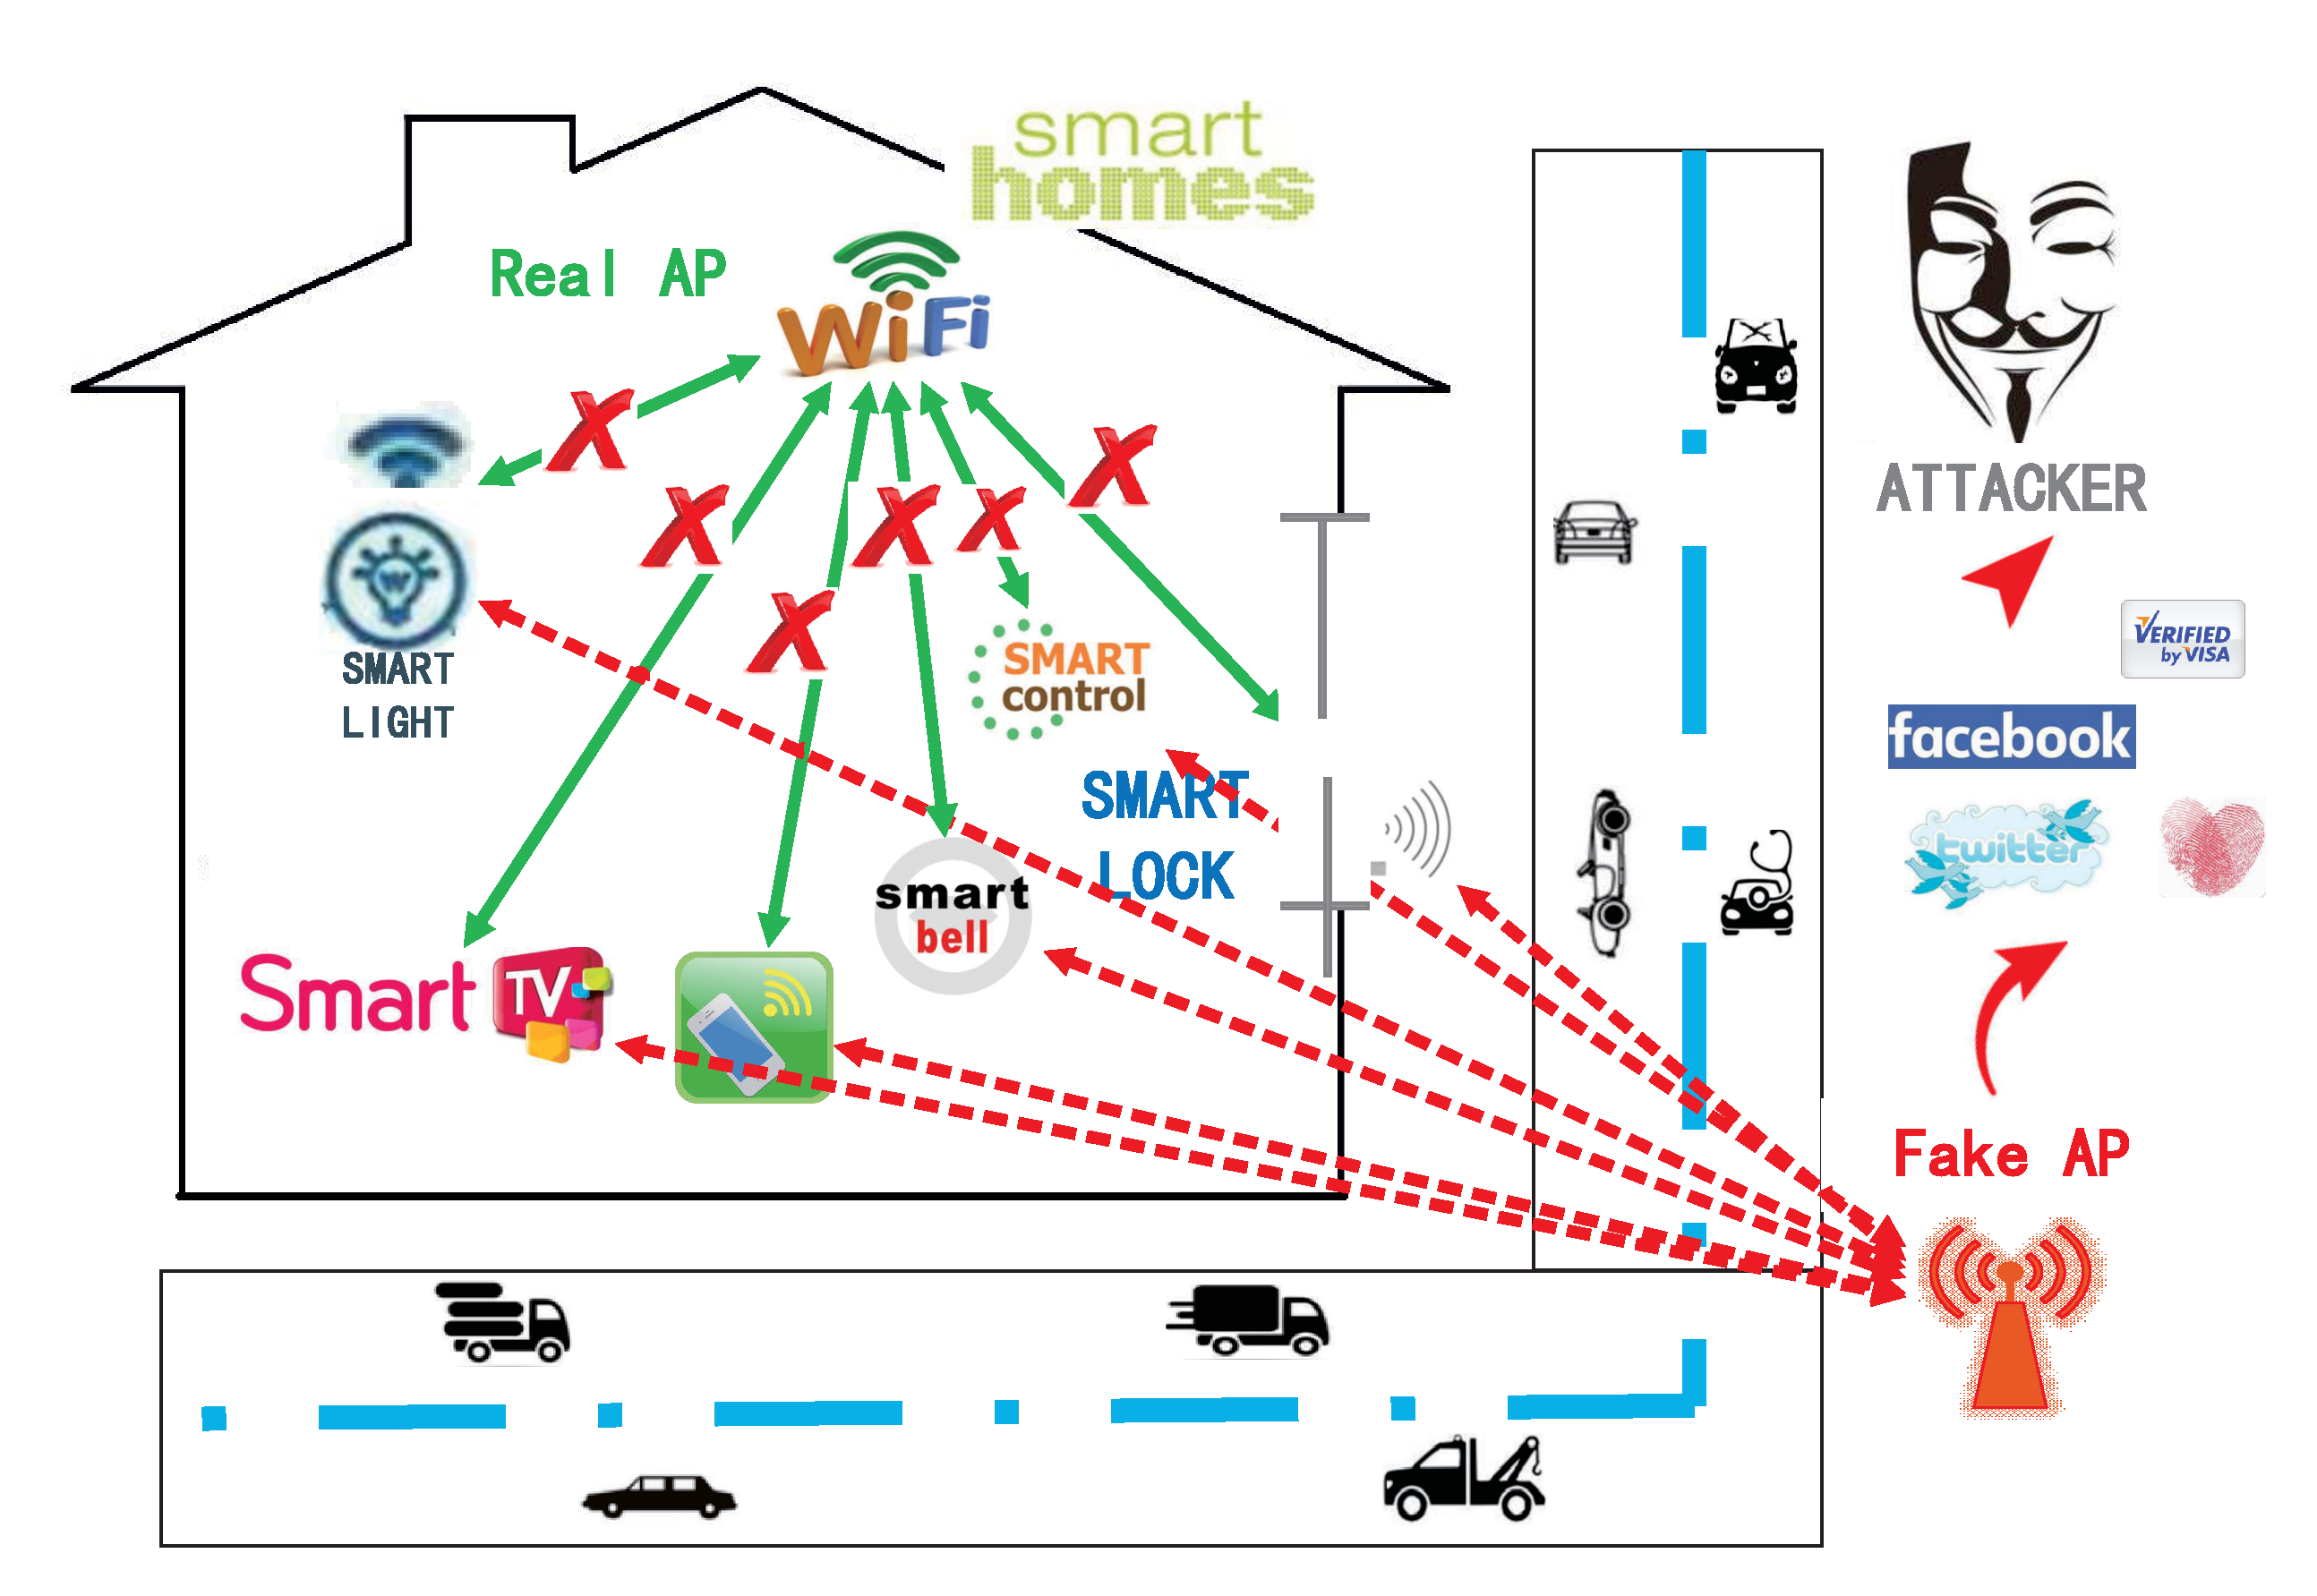
\includegraphics[width=1.0\textwidth]{figure/a}
\caption{Examples scenarios in which the attacker can easily launch an Evil-Twin attack to steal information using a fake AP. This kind of attack typically happens when a hacker constructs a mock (but still functional) Wi-Fi access point (AP) right at the place where there ought to be an original and legitimate Access Point. The reason this works so well is that for a well-orchestrated attack, the illegitimate AP has stronger signals than the legitimate one and hence the unsuspecting users might log on to this mock-up connection and then use the internet while sharing all their precious data -- all the way from their user IDs, passwords to credit/debit card information.}
\end{figure}


\textbf{\secit Attack scenarios}.Figure 1 illustrates the scenarios where the Evil-Twin attack can be applied. Evil Twin (also called WiPhishing) are designed to look like real Wi-Fi hotspots. In those scenarios, the adversary is able to set a Fake AP to launch an Evil Twin attack from a laptop. Its signal might be stronger to the victim than the Real AP. Once disconnected from the legitimate Real AP, the tool then force offline computers and devices to automatically re-connect to the evil twin, allowing the hacker to intercept all the traffic to that device. When people in Smart Homes are using the Internet through an Evil Twin, they can unknowingly expose their passwords and other sensitive online data to hackers. According to the Wi-Fi Alliance, a sophisticated Evil Twin can even control what websites appear when users access the Internet. That allows hackers to capture their passwords.

\textbf{\secit Assumptions}.Our attacks require the adversary to set up the evil twin at a different location. We believe that the adversary maybe not set the Fake AP very close to the Smart Homes in order to avoid being caught. If a profile for the legitimate AP exists, the client device will automatically connect to the faked AP.




\section{DRET  OVERVIEW}
DRET is a system that helps wireless home owner to discover and prevent Evil Access Points (AP) from attacking wireless users. The application can be run in regular intervals to protect your wireless network from Evil Twin attacks. By configuring the tool you can get notifications sent to you alarm signal whenever an evil access point is discovered. Additionally you can configure DRET to perform DoS on the legitimate wireless users to prevent them from connecting to the discovered evil AP in order to give the administrator more time to react. However, notice that the DoS will only be performed for evil APs which have the same SSID but different BSSID (AP's MAC address) or running on a different channel. This to avoid DoS your legitimate network

\begin{figure}[h]
\centering
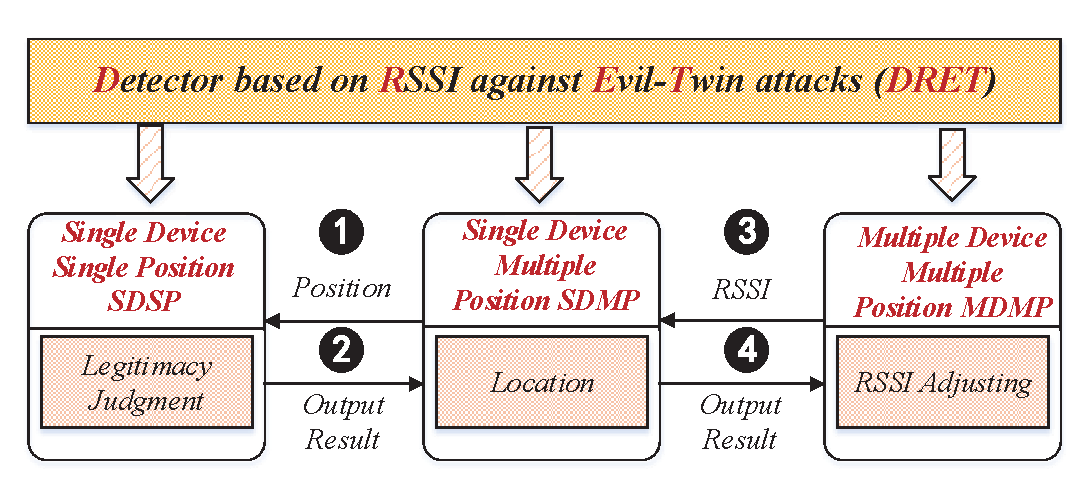
\includegraphics[width=0.85\textwidth]{figure/b}
\caption{The overview of DRET System.DRET mainly consists of three parts (SDSP\&SDMP\&MDMP).}
\end{figure}

Following a common practice in FAKE AP detection, DRET will choose different modular depending on different circumstances. SDSP meet the simple scenario such as during night and when nobody is at home. However, SDSP is limited and the success rate is closely related to the Detector location. To addressing this limitation, SDMP is proposed, which locate the mobile phone firstly, the RSS fingerprint value is drawn to SDSP(\ding{182}), so the SDSP can determine the location of legitimacy(\ding{183}), the result return to SDMP.  Sometimes many devices work in multi places, these devices need to use only one set of fingerprint data to check at the same time. MDMP will start, the RSSI is adjusted and then send to SDMP(\ding{184}), the result done by SDMP return to MDMP(\ding{185}).






\section{PRELIMINARIES}
In order to construct a real environment, the attacker will do anything to improve the Fake AP so that it has the same features a Real AP, including traffic characteristics and hardware fingerprint characteristics. However, the attacker cannot forge the position of the Real AP. In Smart Homes, the intuition underlying our design is that each Real AP has its fixed position, and the attacker cannot put the Fake AP exactly in the right place. Therefore, a new Smart Home Fake AP detected method based on RSSI is proposed in this paper.

 Figure 3 is shown as the principle of Fake AP Detection based on RSSI. RAP and FAP are respectively represented Real AP and Fake AP. Detector receives the signal from each AP. D1 is the distance between the $Detector_{1}$ with the Real AP, and D1' is the distance between the $Detector_{1}$  with the Fake AP. If D1 is greater than D1', it means that the intensity of $Detector_{1}$  received from the Fake AP is stronger than the Real one. In general, when there exists multipath effect, Detector always choose the strongest signal in the homologous signals. So, undoubtedly, when the attacker turn on $FAP_{1}$, $Detector_{1}$  will choose it rather than the real $RAP_{1}$. But when the attacker turn off the $FAP_{1}$, The $Detector_{1}$ will choose RAP. According to the upper analysis, we can easily identify the Fake AP from the Real one by comparing the RSSI of them. In this scene, If $RSSI_{1}$' is greater than $RSSI_{1}$, it means that $FAP_{1}$ is Fake AP.

\begin{figure}[h]
\centering
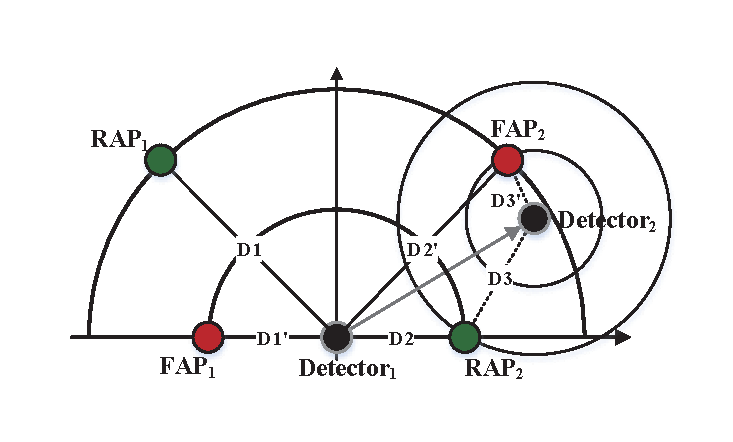
\includegraphics[width=1.0\textwidth]{figure/1}
\caption{The figure shows two REAL APs(in green) and two FAKE APs(in red). The figure illustrates that the Detector(in black)  how to  recognize the  FAP by using the differences of the RSSI that the APs locate differently.
}
\end{figure}


However, there is another scene that the distance between the Real AP and detector is less than the Fake one's. In this condition, no matter open or shutdown the Fake AP, the detector would always choose the Real AP. So, we should try to build a scene like the previous one, namely, moving the detection's position to $Derector_{2}$, making D3' is greater than D3, then we can detect the Fake AP.

In free space, the path loss of signal propagation express signal attenuation, which is defined as the difference value between the effective radiated power and the received power. So the path loss in free space can be computed by the following formula.$G_{t}$ and $G_{r}$ separately express the antenna gain of the sender and the receiver.$\lambda$ indicates the signal wave length, d is the distance between the sender and receiver.

\begin{displaymath}{PL(dB)=10\log \frac{P_{t}} {P_{r}} = -10\log \left[\frac{G_{t}G_{r}\lambda^{2}} {(4\pi)^{2}d^{2}}\right]}(1)
 \end{displaymath}

Frequency of WIFI channel 1$\sim$13 is from 2.412$\ast$$10^{9}$ $\sim$ 2.472$\ast$$10^{9}$. And there exists $\lambda$=c/f, c$\approx$3$\ast$$10^{8}$m/s,so the value range of $\lambda$ is 0.1214 $\sim$0.1244. We did some experiment to study what factors effecting the attenuation and the attenuation curve is shown as the Figure 4. In Figure a, both of the sender and receiver has unity-gain, and the channel is 1. In Figure b, both of the sender and receiver has unity-gain, and the channel is 13. In Figure c, the Antenna gain product of the sender and receiver is 100, and the channel is 13. From the Figure 4, we can find the following rules. (1) From a and b, we can find that the effect of channel on attenuation is very small. (2) From b and c, we can find that antenna gain has a great influence on attenuation. (3) From a, b and c, we can find that the distance is the main factor to affect the attenuation, and the attenuation is less sensitive to the distance with the increase of distance.

\begin{figure}[h]
\centering
\includegraphics[width=1.0\textwidth]{figure/2}
\caption{Signal attenuation curve}
\end{figure}

RSSI (Signal Strength Indicator Received) is the intensity of the received signal, its value can be calculated by the following formula:

RSSI = Transmit Power + Antenna gain - Path Loss

For a fixed transmitter and receiver, the Transmit Power and Antenna Gain are both constant, and the Path Loss is a function of the distance D, so RSSI can be expressed as RSSI=f(d). Then d will be d=f'(RSSI).
 Therefore, RSSI can be used directly to replace the distance for positioning.

In order to be simplify the calculation, we proposed Signal Space and Signal Distance. Signal Distance can be abbreviated as sd, then sd=$\textbar$RSSI$\textbar$. In Figure 5, the left are the physical space, and the right is the signal space. Both of them take AP as the reference point. Point a, b, c, d is the position of four mobile phones. In the physical space, the distance separately between a, c, d are equal, less than the distance between b and AP. But there are obstacles at the point a and d, where the attenuation of the black obstacle is higher than the gray obstacle, so $sd_{a}$$\textgreater$$sd_{d}$$\textgreater$$sd_{c}$,
 $sd_{b}$$\textgreater$$sd_{c}$. In general, the signal strength of straight line is the best when there is no obstacle, and wireless devices always give priority to the best signal when dealing with multipath effects. So, from the physical space to the signal space, the distance of their signal has some slight changes, which is shown as the right figure.

\begin{figure}[h]
\centering
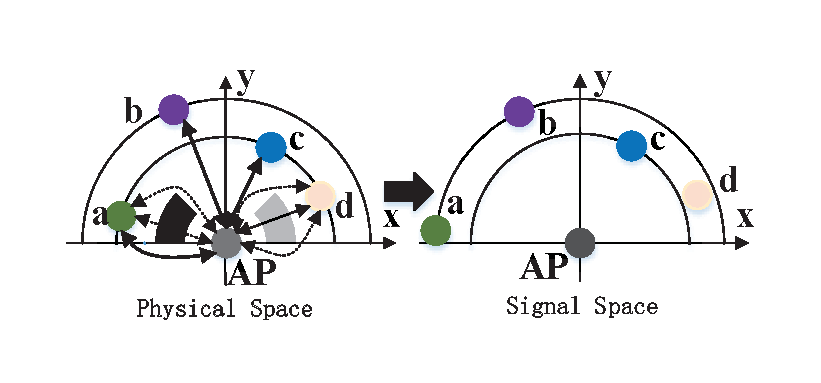
\includegraphics[width=1\textwidth]{figure/3}
\caption{Physical Space convert to Signal Space}
\end{figure}

In order to verify that the RSSI can be used as the defection factor, we did an experiment. In normal circumstances, we build a fingerprint library by using the signal distance. Terminal MX3 is used as director to collect RSSI signal and the TL-WR882N is used as AP. The distance between them are 5m, and data collection rate is 2 times per second. We collected about 14000 of the total data, keeping surrounding environment is not changed during the process of collecting data, except that someone walked across. Its probability distribution histogram is shown as the following figure 6.

\begin{figure}[h]
\centering
\includegraphics[width=1\textwidth]{figure/4}
\caption{probability distribution histogram}
\end{figure}

By analyzing the experiment data, it is found that the measured value of the actual measurement is near to a stable value, and the probability distribution is approximately normal distribution. That means the RSSI can be used as the defection factor.

Actually, it seems that both of the Fake and Real AP is similar to the detector, which are difficult to be distinguished. According to multipath effect, the detector will select the one with the strongest signal to associate and compute the distance between the selected AP and it, which will be compared with the distance recorded in signal distance fingerprint database. If they are different, that means the AP should be forged. The mobile phone will be used as the detector. Depending on whether the mobile phone which be used as a detector in smart home moving or not, two different kinds of solution has been proposed in this paper, they are: a single fixed position detection and the multi-position collaborative detection.

\section{AUTOMATED DETECTION ANALYSIS}
\subsection{\secit A SINGLE FIXED POSITION DETECTION}
Smart homes devices still need work under networking even there is no one at home, the detector is also. Therefore, we install the detector in a fixed position, and let it work 24 hours. Detector establish target AP RSSI fingerprint library in normal sense, which would be used as sample when detecting. Only the detected distance is within the error range of distances recorded in fingerprint database, it is considered as the fake AP, otherwise, it is true AP.

It is assumed that the deployment of hot spot and detector as shown in Figure 7. The position of fake AP and true AP are different, but the other features are same, such as network card hardware features, antenna gain, stability, etc.. A, B, and C are the positions of three detectors. The signal intensity of true AP and fake AP is the same in the position A (shown as Y2 axis). The signal intensity of true AP is stronger than ones of fake AP in the position B, and the opposite in position C.

\begin{figure}[h]
\centering
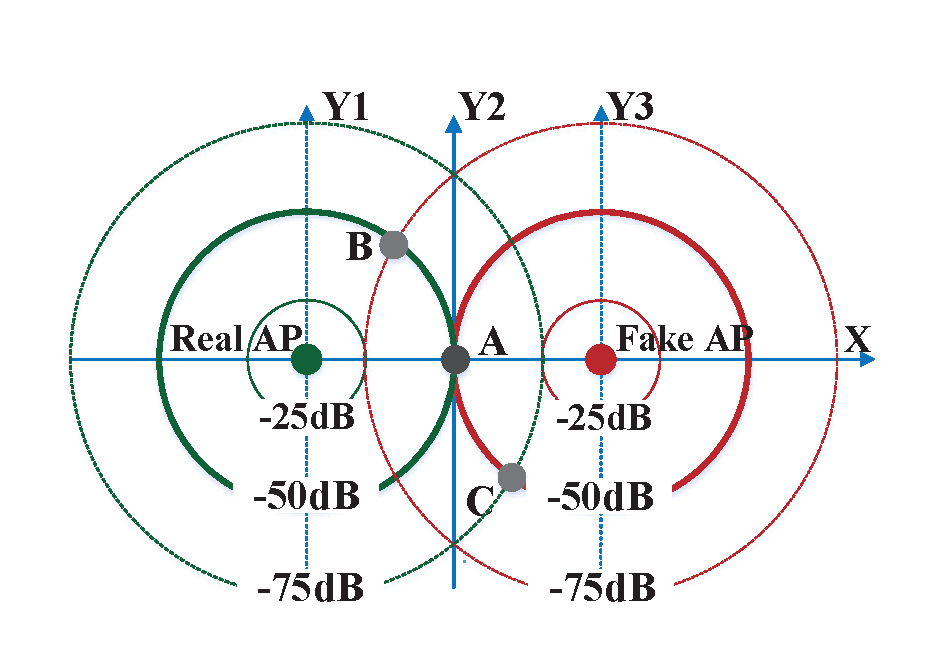
\includegraphics[width=1\textwidth]{figure/5}
\caption{A single fixed position detection}
\end{figure}

In the security state, that is, where there not exits the fake AP, the RSSI and variance of signal intensity which separately received by three detectors at position A, B, C is shown in the following form.

\begin{table}[h]
\centering
\caption{FSSI and Variance in the security State}
\begin{tabular}{|c|c|l|} \hline
Location&Average&Variance\\ \hline
A & $\mu_{A}$=-50& $\sigma_{A}$\\ \hline
B & $\mu_{B}$=-50& $\sigma_{B}$\\ \hline
C & $\mu_{C}$=-75& $\sigma_{C}$\\ \hline
\end{tabular}
\end{table}

Fake AP's working will lead to multipath effect. Therefore, it is assumed that PA,PB,PC is the probability of selecting true AP signal in A, B, C. Under ideal conditions,
0$\textless$=$P_{C}$$\textless$$P_{A}$=0.5$\textless$$P_{B}$$\textless$=1 , and the new Average and Variance is shown as the following form. Both of them wave in a certain range of fluctuation due to kinds of factors like the multipath effect, the external interference and etc.. It is assumed that the Average an Variance meeting the following conditions, ,$\mu$-M$\textless$=$\mu$$\textless$=$\mu$+M,$\sigma$$\textless$=$\Sigma$ .

\begin{table}[h]
\centering
\caption{FSSI and Variance when fake AP is working}
\begin{tabular}{|c|c|l|} \hline
Location&Average&Variance\\ \hline
A & $\mu'_{A}$=$\mu_{A}$=-50& $\sigma'_{A}$=$\sigma_{A}$\\ \hline
B & -75$\textless$$\mu'_{B}$$\textless$-50& $\sigma'_{B}$$\textgreater$$\sigma_{B}$\\ \hline
C & -75$\textless$$\mu'_{C}$$\textless$-50& $\sigma'_{C}$$\textgreater$$\sigma_{C}$\\ \hline
\end{tabular}
\end{table}

From figure 7, we can see that when the detector in region C, it will select Fake AP since whose signal intensity is stronger than the Real AP's, which can be described with the formula like $\mu'$$\textgreater$$\mu$.When $\mu'$$\textgreater$$\mu$+M, we can say that there exists a Fake AP in the network. When the detector in region A,$\mu'$=$\mu$, that means we cannot distinguish the Real AP and the fake one. In region B, although the signal intensity of Real AP is higher than Fake AP, but the detector considers both of them is the same signal, the latter is still cannot be detected.

As analysis shows, detector and Real AP cannot be too close that will lead to high misdetection rate, so the best deployment location of detector is in region C where the signal is weak, far away from the Real AP and near the Fake AP.
\subsection{\secit MULTI POSITION DETECTION}
Obviously, a single fixed position detection method can only solve part of the problem. In this part, multi position detection is proposed. Multi position detection relies on mobile phones, with it we can convert multi position to single fixed position detection. So, first what we need to do is determining the position of the mobile phone. The most well-known and high accuracy of the positioning method is GPS, while GPS devices have been known to not work very well indoors. In this paper, we use the WIFI signal for locating the position of mobile phone by Three point positioning method. With the popularity of WIFI, there are almost always more than three WIFI hotspots will be found when we are indoors.

\begin{figure}[h]
\centering
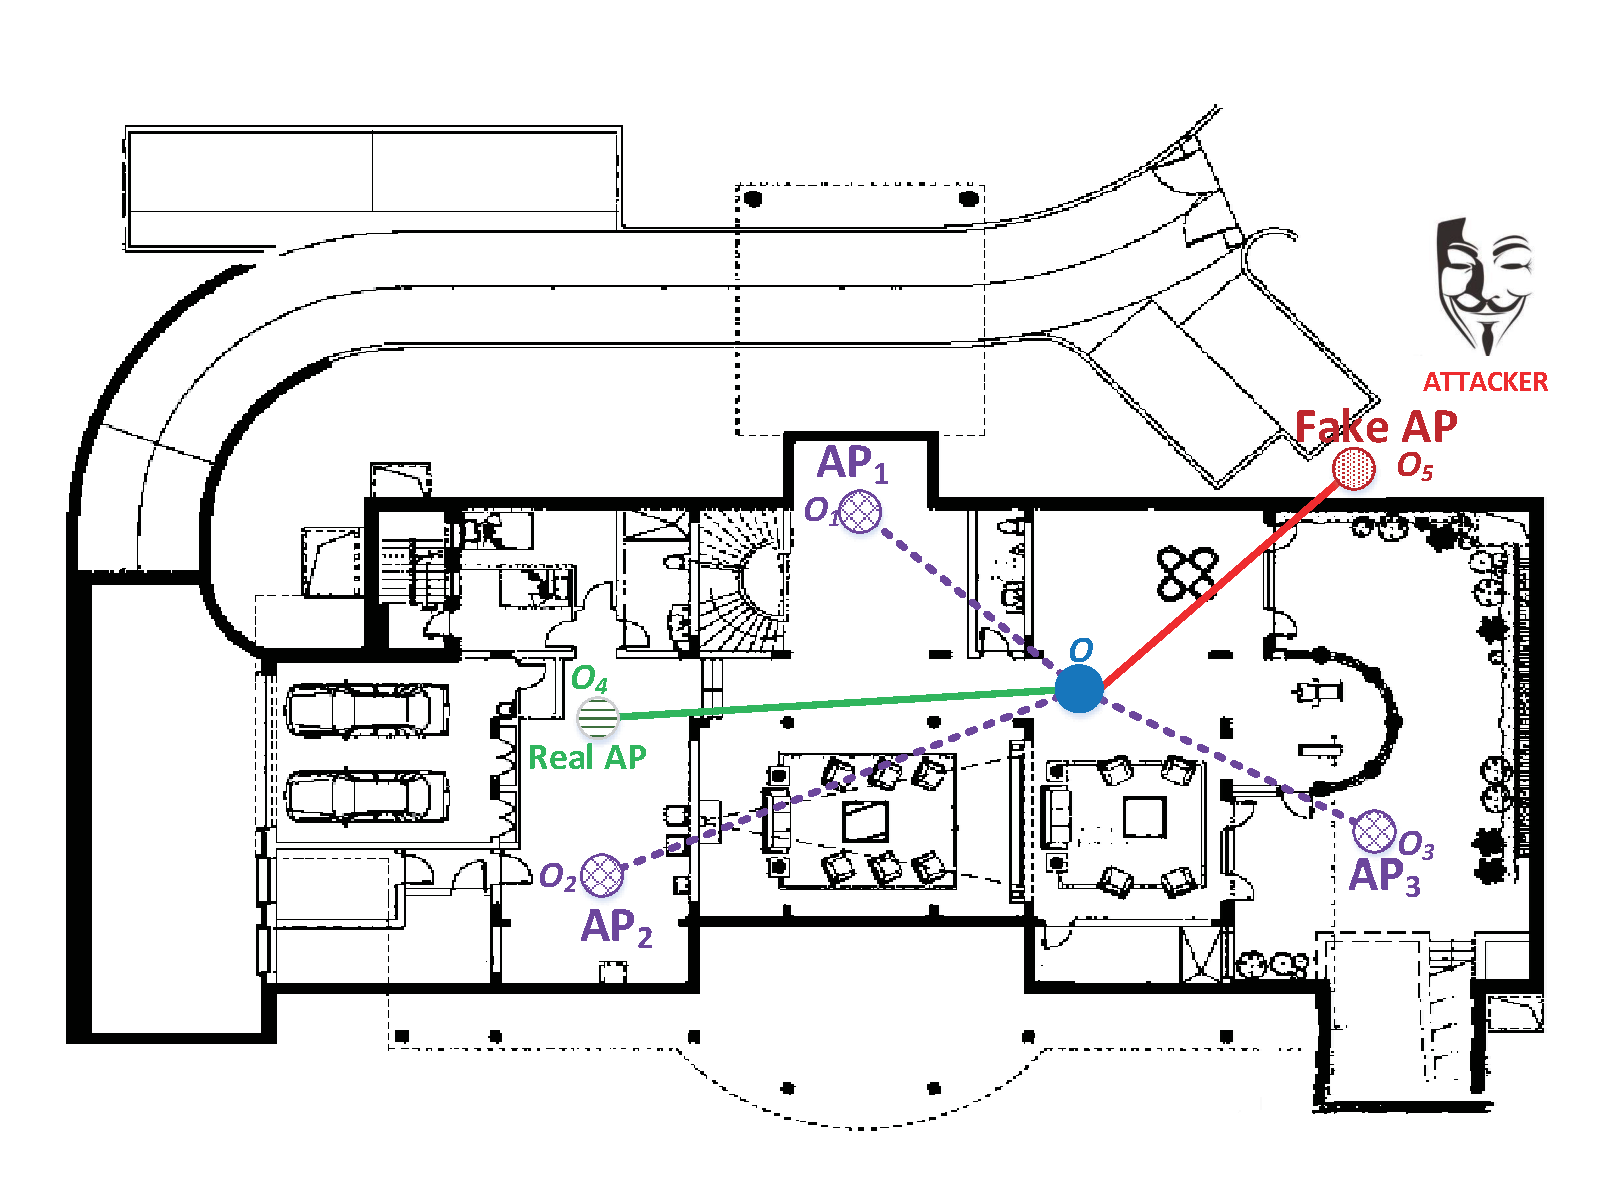
\includegraphics[width=1\textwidth]{figure/6}
\caption{Multi position Detection transformation. The figure show that any three APs could be choosed as reference in the signal space. They are used to loacate the positions of the MobilePhone which is a detector in Smart Homes.}
\end{figure}

As shown in Figure 8, $AP_{1}$,$AP_{2}$and $AP_{3}$ are three different APs, assuming their positions are known. O is the mobile phone's position. The original distance can be defined as sd which represents the distance between AP and mobile phone.$sd_{i}$=$\textbar$$OO_{i}$$\textbar$, i=1,2,3,4,5. So $AP_{1}$, $AP_{2}$ and $AP_{3}$ can locate the position of the mobile phone in the signal space. Then we can convert the Multi position detection to a Single fixed position detection.

There are two stages in Multi position cooperative detection: fingerprint gathering stage and detection stage. The first stage should be done in a safe state, we collect the RSSI information both of reference AP and target AP in many different positions, to build a fingerprint library. In the detection stage, using reference AP to locate the phone and the fingerprint data in a single fixed position detection, the program framework is shown in figure 8, we can locate the mobile phone's position by using reference AP, then using the method mentioned in the previous chapter to detect.

\begin{figure}[h]
\centering
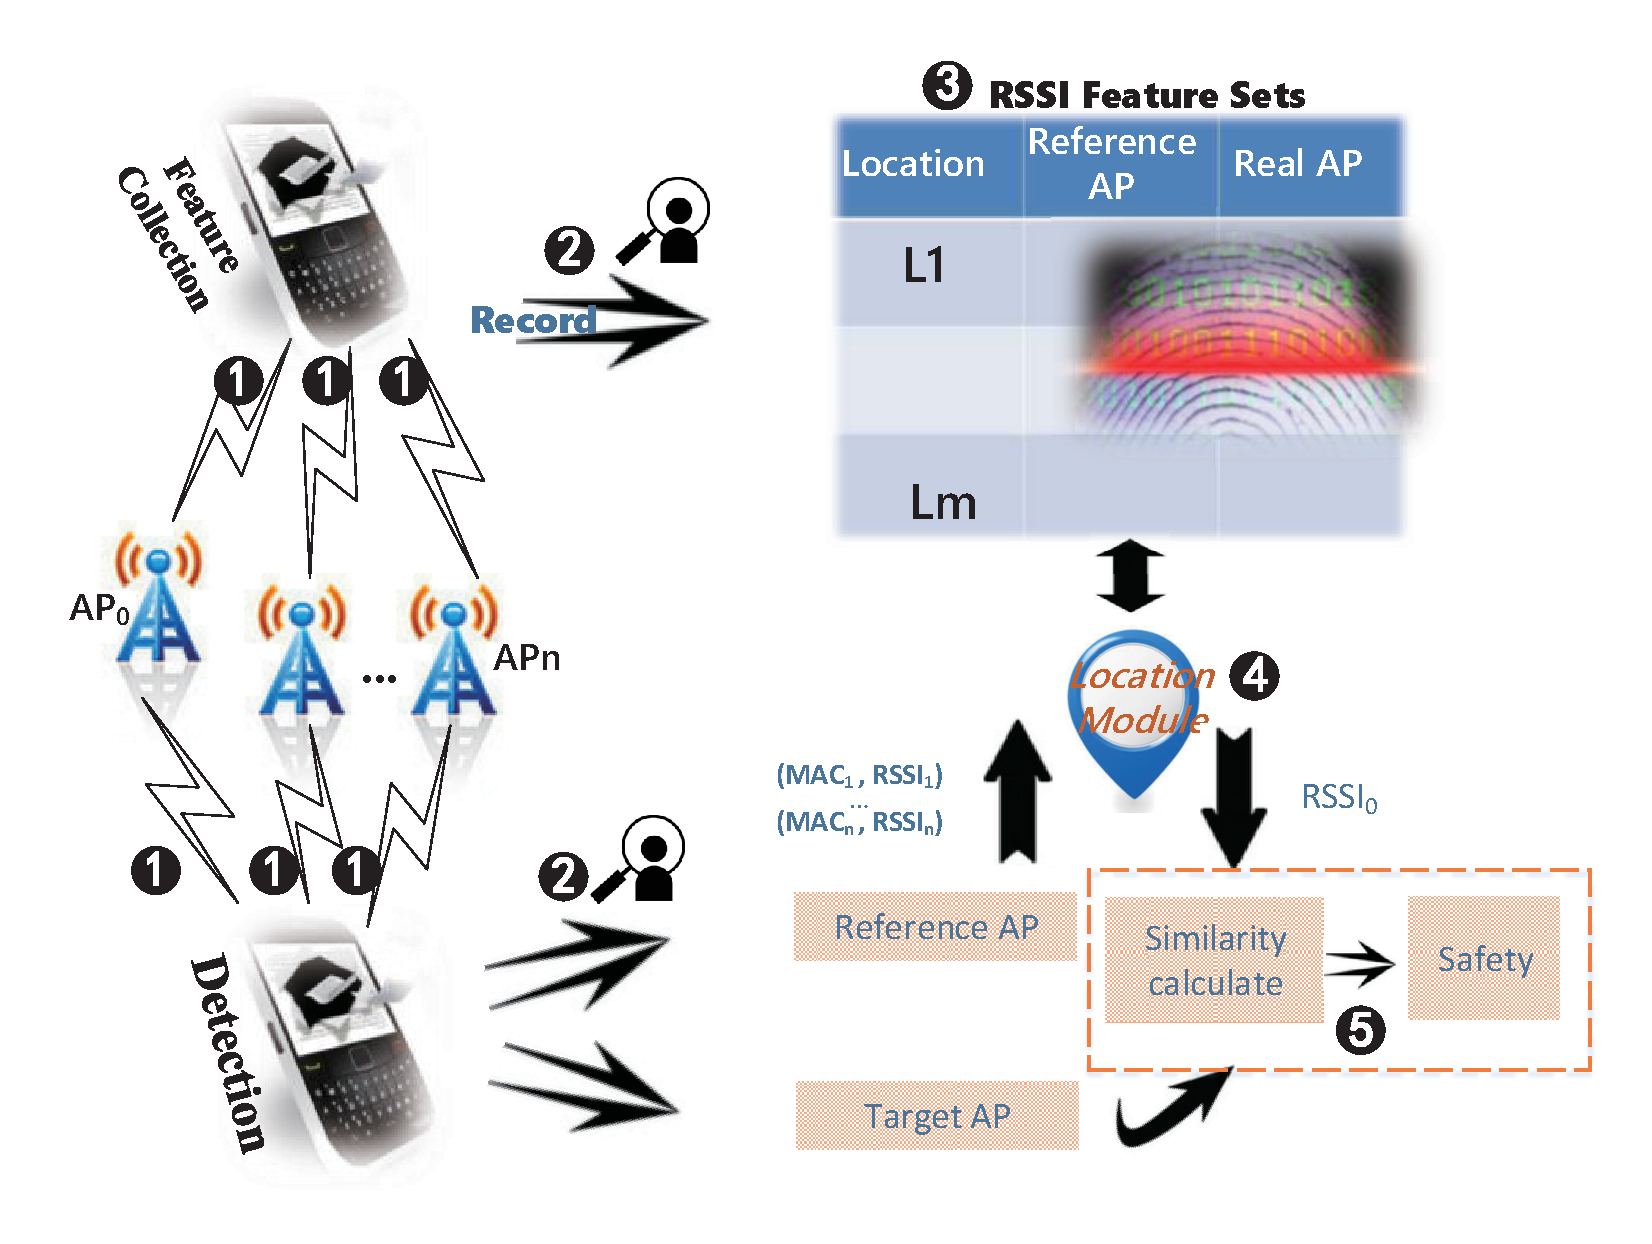
\includegraphics[width=1\textwidth]{figure/7}
\caption{Multi position Detection framework}
\end{figure}

In Figure 9, $AP_{0}$ is the target AP,$AP_{2}$$\sim$$AP_{n}$ are the candidate's reference AP, the whole process can be divided into the following 5 steps:

Step \ding{182}: RSSI acquisition

Step \ding{183}: Effective data selection

Step \ding{184}: Establishment of fingerprint database

Step \ding{185}: Mobile position determination

Step \ding{186}: Validity judgment

\subsubsection{\secit RSSI Acquisition}
In the experiment, the value of RSSI is collected by the interface (IOS: Android:android.net.WIFI. * (SystemConfiguration/CaptiveNetwork.h) in mobile phone .

\subsubsection{\secit Effective Data Selection}
\textbf{Effective RSSI Values Selection}

It is a challenging job to choose the right RSSI values since the mobile phone are always moving. However the RSSI value we need should be waved in a small range, which is shown as the Figure 10.
The data in two boxes are what we want, the others are generated by mobile phone when it is moving. In the condition that the distance between mobile phone and AP is 1m and there is no interference, which generating the data in the first box. Data in the second box is generated in the condition that the distance between mobile phone and AP is 4m and there are two source of interference. The other data is generated in the condition that someone take the mobile phone go around the house with the speed of 1.5m/s.

\begin{figure}[h]
\centering
\includegraphics[width=1\textwidth]{figure/8}
\caption{RSSI Sequence}
\end{figure}

In the first experiment, Variance increment method is used to judge whether the mobile phone is moving. It is assumed that the size of sliding window is 120. When the amount of data is less than the window, it is invalid data.

\begin{displaymath}{W_{i}=\left\{r_{i-ws+1},r_{i-ws+2}...r_{i-1},r_{i}\right\} i\textgreater=ws,r_{i}\in R}
\end{displaymath}

R is the whole RSSI sequence, $r_{i}$ is the value of RSSI, ws is the window size.

The variance can be used to measure the deviation between the RSSI data and the mean value of the window. The variance of $W_{i}$ is $\sigma_{i}$ which express the data fluctuation of $W_{i}$. The greater the data fluctuation, the greater the variance.

\begin{figure}[h]
\centering
\includegraphics[width=1\textwidth]{figure/9}
\caption{RSSI Sequence variance}
\end{figure}

As shown in Figure 11, the window size is 120, two peaks in the middle corresponding to the moving process, that is, it corresponds to the parts not in that two boxes in Figure 10. However, the cause of the big variance is not necessarily a person's movement, the stability of the signal will also affect it. Therefore, the slope of the variance curve is used to determine whether the current is moving. The variance increment K(i).

\begin{displaymath}{k(i)=\frac{d_{\sigma_{i}}} {d_{i}} = \frac{\sigma_{i}-\sigma_{i-1}} {i-(i-1)}=\sigma_{i}-\sigma_{i-1}}(3)
 \end{displaymath}

In Formula 3,$\sigma_{i}$ is the variance of $W_{i}$,$\sigma_{i-1}$ is the variance of $W_{i-1}$.

\begin{figure}[h]
\centering
\includegraphics[width=1\textwidth]{figure/10}
\caption{RSSI Sequence variance}
\end{figure}

The results of improved is shown in Figure 12. When k(i) is near to 0, it means that the original variance is stable in a certain range, that also means the mobile phone is not moving or moving in a small range. We set a threshold to detect whether the mobile phone is moving. If $\textbar$k(i)$\textbar$$\textless$=K, the mobile phone is considered to be stable, otherwise it means the position of mobile phone has changed.

Those sequence with a stable position has the following characteristics:

Start point:[$\textbar$k(i)$\textbar$$\textless$=K]-ws(+1)

End point:[$\textbar$k(i)$\textbar$$\textgreater$K]-ws/2

\textbf{Effective reference AP selection}

In order to improve the accuracy of multi position detection, it is needed to improve the accuracy of the location. Because of the complexity of the wireless signal transmission in the indoor environment, the AP signal is not stable. In the network environment, a position can be detected more than one AP. Therefore, Signal stability and the relevance with target AP are the two factors in choosing AP. Relevance here means that both the target AP and the reference AP moving with the mobile phone, that's why the fluctuations of the variance between the target AP and the reference AP should be consistent.

We use Dynamic (Time Warping DTW\cite{Wang}, dynamic time warping) algorithm to calculate the distance and determine the validity of the reference AP. DTW is a method that calculates an optimal match between two given sequences (e.g. time series) with certain restrictions. The sequences are "warped" non-linearly in the time dimension to determine a measure of their similarity independent of certain non-linear variations in the time dimension. This sequence alignment method is often used in time series classification.

As shown in Figure 13, picture on top calculate distance without using dynamic time but the below one uses, it can make calculation of the distance reaching the minimum distortion.

\begin{figure}[h]
\centering
\subfloat[]{
\label{fig:subfig:}
\includegraphics[width=0.8\textwidth]{figure/d}}
\hspace{1in}
\subfloat[]{
\label{fig:subfig:}
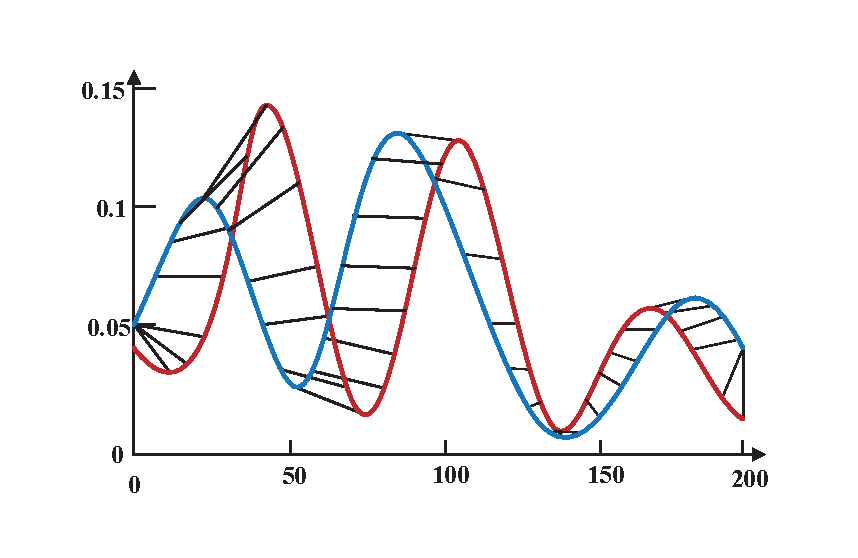
\includegraphics[width=0.8\textwidth]{figure/c}}
\caption{dynamic time warp (DTW)}
\label{fig:subfig}
\end{figure}



When selecting the effective reference AP, each AP is considered as the candidate reference AP. The large number of its variance increment is stored and the distance between its variance increment sequence and the target's. After getting the distance of all candidate reference APs and target APs, all candidate reference APs will be ordered by the distance. The smaller the distance, the better the effectiveness. Therefore, four candidate reference APs with the minimum distance will be choose as the reference APs to locate the mobile phone's position. In general, three points are enough for location. In order to prevent that one of the three reference APs is failure, so we choose four reference APs from the candidate lists.

\subsubsection{\secit Establishment of Fingerprint Database}
The RSSI fingerprint Library (RSSI-MAP) is built by the RSSI sequence generated in previous section. RSSI-MAP is shown in Form3. $R_{J}$=($r_{1,J}$,$r_{2,J}$...$r_{L,J}$)represent the fingerprint information in RSSI-MAP. J is the position where the mobile phone is stayed for detecting. L is the number of candidate reference APs. r is the fingerprint information of AP, which can be described by triple like r($\overline{rssi}$,var,len). Items in triple represents the average, variance and length of RSSI sequence.

\begin{table}[h]
\centering
\caption{structure of RSSI-MAP}
\begin{tabular}{|c|c|l|} \hline
Location&Reference AP&Target AP\\ \hline
1 & $R_{1}$=($r_{1,1}$,$r_{2,1}$...$r_{L,1}$)& $R'_{1}$=$r_{0,1}$\\ \hline
2 & $R_{2}$=($r_{1,2}$,$r_{2,2}$...$r_{L,2}$)& $R'_{2}$=$r_{0,2}$\\ \hline
... & ...& ...\\ \hline
J & $R_{J}$=($r_{1,J}$,$r_{2,J}$...$r_{L,J}$)& $R'_{J}$=$r_{0,J}$\\ \hline
\end{tabular}
\end{table}

\subsubsection{\secit Mobile Position Determination}
$R_{T}$=($r_{1,T}$,$r_{2,T}$...$r_{L,T}$) represents RSSI fingerprinting information of the reference APs are detected at the position T.$R'_{T}$=$r'_{0,T}$ represents the RSSI fingerprinting information of the target AP is detected by the position T.Dist($R_{T}$,$R_{J}$)is the distance between $R_{T}$ and $R_{J}$.$\overline{rssi_{i,T}}$ is the average value of RSSI for reference AP,$\overline{rssi_{i,J}}$ is the average of the RSSI sequence for reference AP. j is the position where the distance between T and one in RSSI-MAP is the shortest. When there are more than three reference APs, we can locate the mobile phone.

%��ʽ��4��
\begin{displaymath}{Dist(R_{T},R_{J})=\sqrt{\sum_{i=1}^{L}(\overline{rssi_{i,T}}-\overline{rssi_{i,J}})^{2}}}(4)
 \end{displaymath}

Dist($R_{T}$,$R_{J}$) in Formula 4 depend on the number of L, in order to reduce the effect on $Dist_{T}$ that the number of reference AP are different in different position. The formula is improved as the following.

%��ʽ��5��
\begin{displaymath}{Dist_{T}=min\left[\frac{Dist(R_{T},R_{J})} {L}\right]}(5)
 \end{displaymath}

When L is greater than or equal to 3, the fingerprint of the first three APs can be used to location by using Formula 4 and 5. When L is equal to 2, there will be more than one position and all of them have the same distance. Then we should choose the one who is the nearest one with the target AP. When L is equal to 1, in order to increase the accuracy of the positioning, the variance is used to measuring the similarity between position T and position J. From the previous section, the RSSI form one AP at the same position is approximate normal distribution, that is, the RSSI sequence is represented as follows:

%��ʽ��6��
\begin{displaymath}{P(rssi)=\frac{1} {\sqrt{2\pi}\sigma}e^{\frac{(rssi-\mu)^{2}}{2\sigma^{2}}}}(6)
 \end{displaymath}

In Formula 6,$\sigma$=var,$\mu$=$\overline{rssi}$.

In the information theory, KL\cite{2307,kullback1987letter} Kullback (Leibler - divergence) can be used to describe the difference between two probability distributions of Q and P,$D_{KL}$(P$\textbar\textbar$Q) is the information loss caused by that Q is used to fit the true distribution P. So the distance between the T and the RSSI probability distribution can be calculated using the KL divergence. KL divergence is defined as the formula 7.

%��ʽ��7��
\begin{displaymath}{D_{KL}(P\textbar\textbar Q)=\sum P(i)ln\frac{P(i)}{Q(i)}}(7)
 \end{displaymath}

So, we can get formula 8 from formula 6 and formula 7.

%��ʽ��8��
\begin{displaymath}{Dist(R_{T},R_{J})=D_{KL}(R_{T} \textbar\textbar R_{J})=}
 \end{displaymath}

 \begin{displaymath}{\sum_{rssi=-100}^{0}\frac{P(rssi)}{2}\left[\frac{(rssi-\mu_{1})^{2}} {\sigma_{1}^{2}}-\frac{(rssi-\mu_{2})^{2}} {\sigma_{2}^{2}}\right]}(8)
 \end{displaymath}

In the formula 8,$\sigma_{1}$=$var_{L,T}$, $\mu_{1}$=$\overline{rssi_{L,T}}$

\begin{displaymath}{\sigma_{2}=var_{L,J}, \mu_{2}=\overline{rssi_{L,J}}}
\end{displaymath}

%��ʽ
\begin{displaymath}{P(rssi)=\frac{1} {\sqrt{2\pi}\sigma_{1}}e^{\frac{(rssi-\mu_{1})^{2}}{2\sigma_{1}^{2}}}}
 \end{displaymath}

Then, according to the distance got by formula 8, the nearest neighbor algorithm is used to find the corresponding position in the J RSSI-MAP.

\subsubsection{\secit Legitimacy Judgment}
max($\overline{rssi}$)represents the maximum mean of target RSSI at position J. It is can be easily query in RSSI-MAP when we find the position J. $\overline{rssi}$ is the mean value being detected. Then, there is $Diff_{T}$=$\overline{rssi}$-max($\overline{rssi}$).

If $Dist_{T}$$\textless$=M and $Diff_{T}$$\textless$=0, safe and there is no fake AP.

If $Dist_{T}$$\textless$=M and $Diff_{T}$$\textgreater$0, unsafe and there exits fake AP:

If $Dist_{T}$$\textgreater$M, fingerprint database should be updated. You can find the details in next section.

\subsubsection{\secit Dynamic Update of Fingerprint Database}
The dynamic update of RSSI fingerprint database consists of two parts, one is the addition of the new fingerprint, and the other is the update of the existing fingerprint.

The new fingerprint should be added is because of various reasons in the training phase of the RSSI fingerprint database. It can't cover all the spatial sub regions of M, so it is necessary to improve the fingerprint database in the later stage.

The update of the existing fingerprint is caused by environmental changes such as survival status of reference AP, the correlation between the candidate reference AP and the target AP, the change of the reference AP's position and so on. At this point, we need to update the fingerprint information which has already exists in the fingerprint database in detection stage.
\begin{displaymath}{\left[R_{J}\left(r_{1,J},r_{2,J}...r_{L,J}\right),R'_{J}\left(r_{0,J}\right)\right]}
\end{displaymath}

%��ʽ
Assume there are four valid candidate reference AP, they are $AP_{1}$,$AP_{2}$,$AP_{3}$,$AP_{4}$, and the relationship or their effectiveness is as the following: E1>E2>E3>E4,then there is $Dist_{T}$=$Dist_{T}$($AP_{1}$,$AP_{2}$,$AP_{3}$), The corresponding position is J.

When there is $Dist_{T}$$\textgreater$M
%��ʽ
\begin{equation} \left\{ \begin{aligned} \overset{.}Dist_{T3} &=Dist_{T}\left(AP_{1},AP_{2},AP_{4}\right) \\  Dist_{T2}&=Dist_{T}\left(AP_{1},AP_{3},AP_{4}\right) \notag \\
Dist_{T1}&=Dist_{T}\left(AP_{2},AP_{3},AP_{4}\right) \end{aligned} \right. \end{equation}

If $Dist_{Ti}$$\textless$=M, then we can use $r_{i,T}$ instead $r_{i,J}$ in the RSSI-MAP to update the existing fingerprint. If $Dist_{Ti}$$\textgreater$M, then put ($R_{T}$,$R'_{T}$) into the RSSI-MAP. If $Dist_{Ti}$$\textless$=M and $r_{i,t}$len$\textgreater$=$r_{i,j}$len, then we can use $r_{i,T}$ instead $r_{i,J}$ in the RSSI-MAP.






\section{EVALUATION IN SPD AND MPD}
In order to verify the feasibility and effectiveness of the AP Evil-Twin detection method based on RSSI, we implement a number of experiments.

\subsection{\secit Experiment and Assessment for Single Position Detection}
\textbf{Discussion of Sliding Window Size}

The previous section shows, the size of the sliding window affects the delay rate and false negative rate of detection. That means, the bigger the window, the higher the delay rate is, and the higher the false negative rate is. In order to find a suitable value for the size of sliding window, wo design a experiment like the following.

In order to verify the effect of window size on the delay, we set the mean difference respectively between the fake AP and the true RSSI is 25 and 10, that is, F-R=25 and F-R=10.The window size in turn is: 1, 40, 80, 120, 160, 200, 240. The safety threshold value for each round of detection is the maximum mean of RSSI in 30 minutes. There are 14 sets of experiment, each set of experiment will be done at 30 times, and the result is as showing in Figure 14. From the left figure we can see that when the difference of mean between true AP and fake AP is bigger, the delay rate is smaller. When the window size is 120, the average delay time is less than 20s.

%\begin{figure}[h]
%\centering
%\subfloat[]{
%\label{fig:subfig:}
%\includegraphics[width=0.8\columnwidth]{12-1}}
%\hspace{1in}
%\subfloat[]{
%\label{fig:subfig:}
%\includegraphics[width=0.8\columnwidth]{12-2}}
%\caption{Effect of window size on delay and accuracy}
%\label{fig:subfig}
%\end{figure}

\begin{figure}[htbp]
  \centering
  \begin{floatrow}
     \subfloat[]{
     \begin{minipage}[h]{0.45\linewidth}
         \centering
         \includegraphics[width=1\columnwidth]{figure/12-1}
     \end{minipage}
     }
     \subfloat[]{
      \begin{minipage}[h]{0.45\linewidth}
         \centering
         \includegraphics[width=1\columnwidth]{figure/12-2}
      \end{minipage}
     }
    \end{floatrow}
    \caption{Effect of window size on delay and accuracy}\label{Fig:bufferCon}
\end{figure}




To verify the effect of window size on accuracy, when it is in the condition that F-R=10, we set the windows size in turn: 1, 40, 80, 120, 160, 200, 240. After the test program running 10 minutes, open the fake AP and let it run for 3 minutes then close it for 3 minutes. Because it need a certain delay that the mean value is changed from abnormal status to normal status.

Due to the mean from abnormal status returned to normal needs a certain delay, so every 3 minutes spent after a delay time again wrong inspection or missed, it is assumed that the error detection. If there is wrong or missed detecting after delayed time, it is considered as the error status. This experiment is done 50 times, and the result is shown in the right of Figure 14. According to the experiment results, when the window size is 80, 120 and 160, the accuracy is more than 98\%. If the windows size is too small or too bigger, the accuracy is lower since the false positive rate is higher.

\textbf{Discussion of threshold value}

In this experiment, we set the window size is 120 and the F-R is 25 or 10. Assume that the threshold value is Rmax, Rmax-2, Rmax+2, Rmax+4, Rmax+8. So there are 10 sets of experiment. In each experiment is be done as the following step 50 times. After the test program running 10 minutes, open the fake AP and let it run for 3 minutes then close it for 3 minutes. We can get the result of this experiment from Figure 15, when the security threshold value is Rmax, the accuracy is up to 96\%. When the security threshold value is Rmax+2 , the accuracy of the condition that F-R=25 is up to 100\%, and F-R=25 is 99\%.



\begin{figure}[h]
\centering
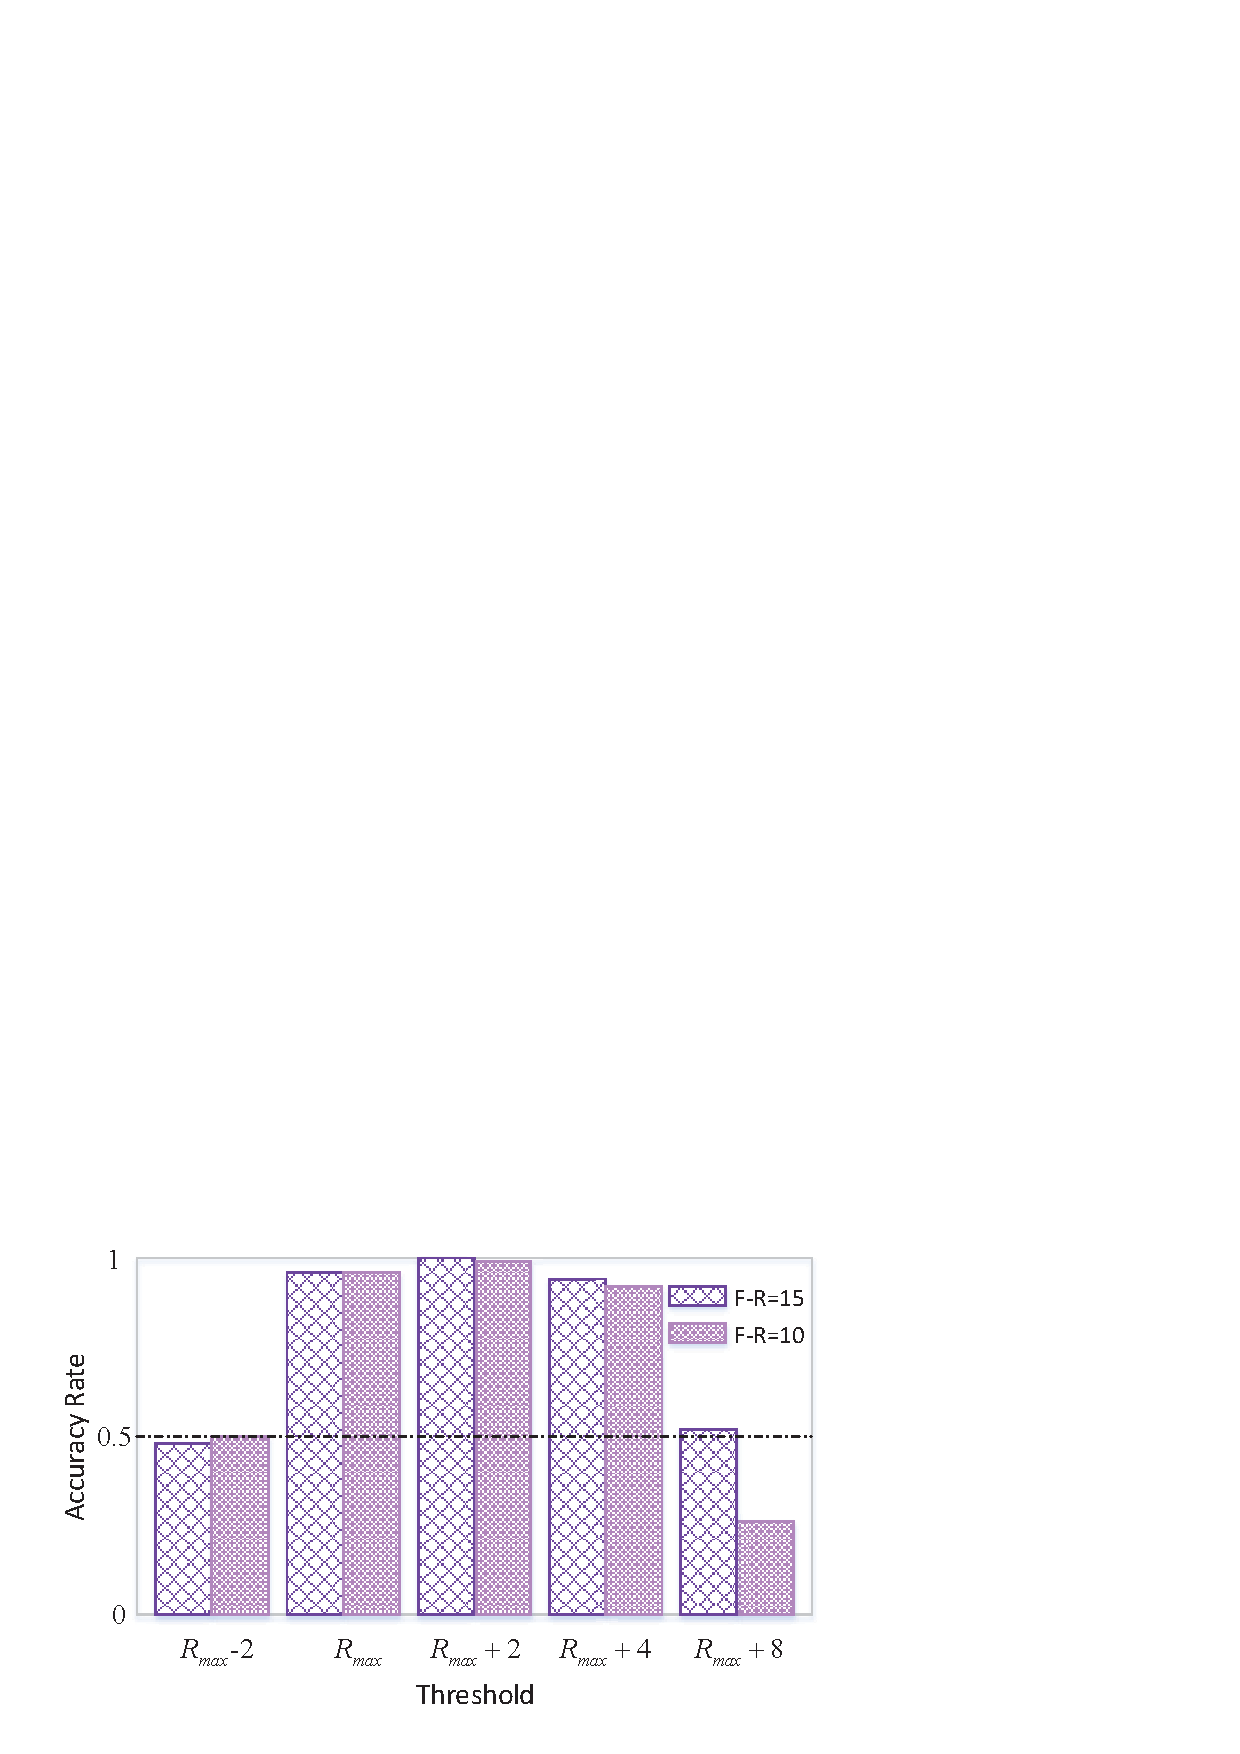
\includegraphics[width=1\textwidth]{figure/13.pdf}
\caption{Effect of safety threshold on the accuracy of detection}
\end{figure}

\textbf{Discussion of distance}

In this experiment, we set F-R=0,5,10,15,20, and the threshold value is Rmax. In each experiment is be done as the following step 50 times. After the test program running 10 minutes, open the fake AP and let it run for 3 minutes then close it for 3 minutes. We can get the result of this experiment from Figure 16. When F-R = 10, the accuracy is more than 96\%, the missing rate is less than 3\%.

\begin{figure}[h]
\centering
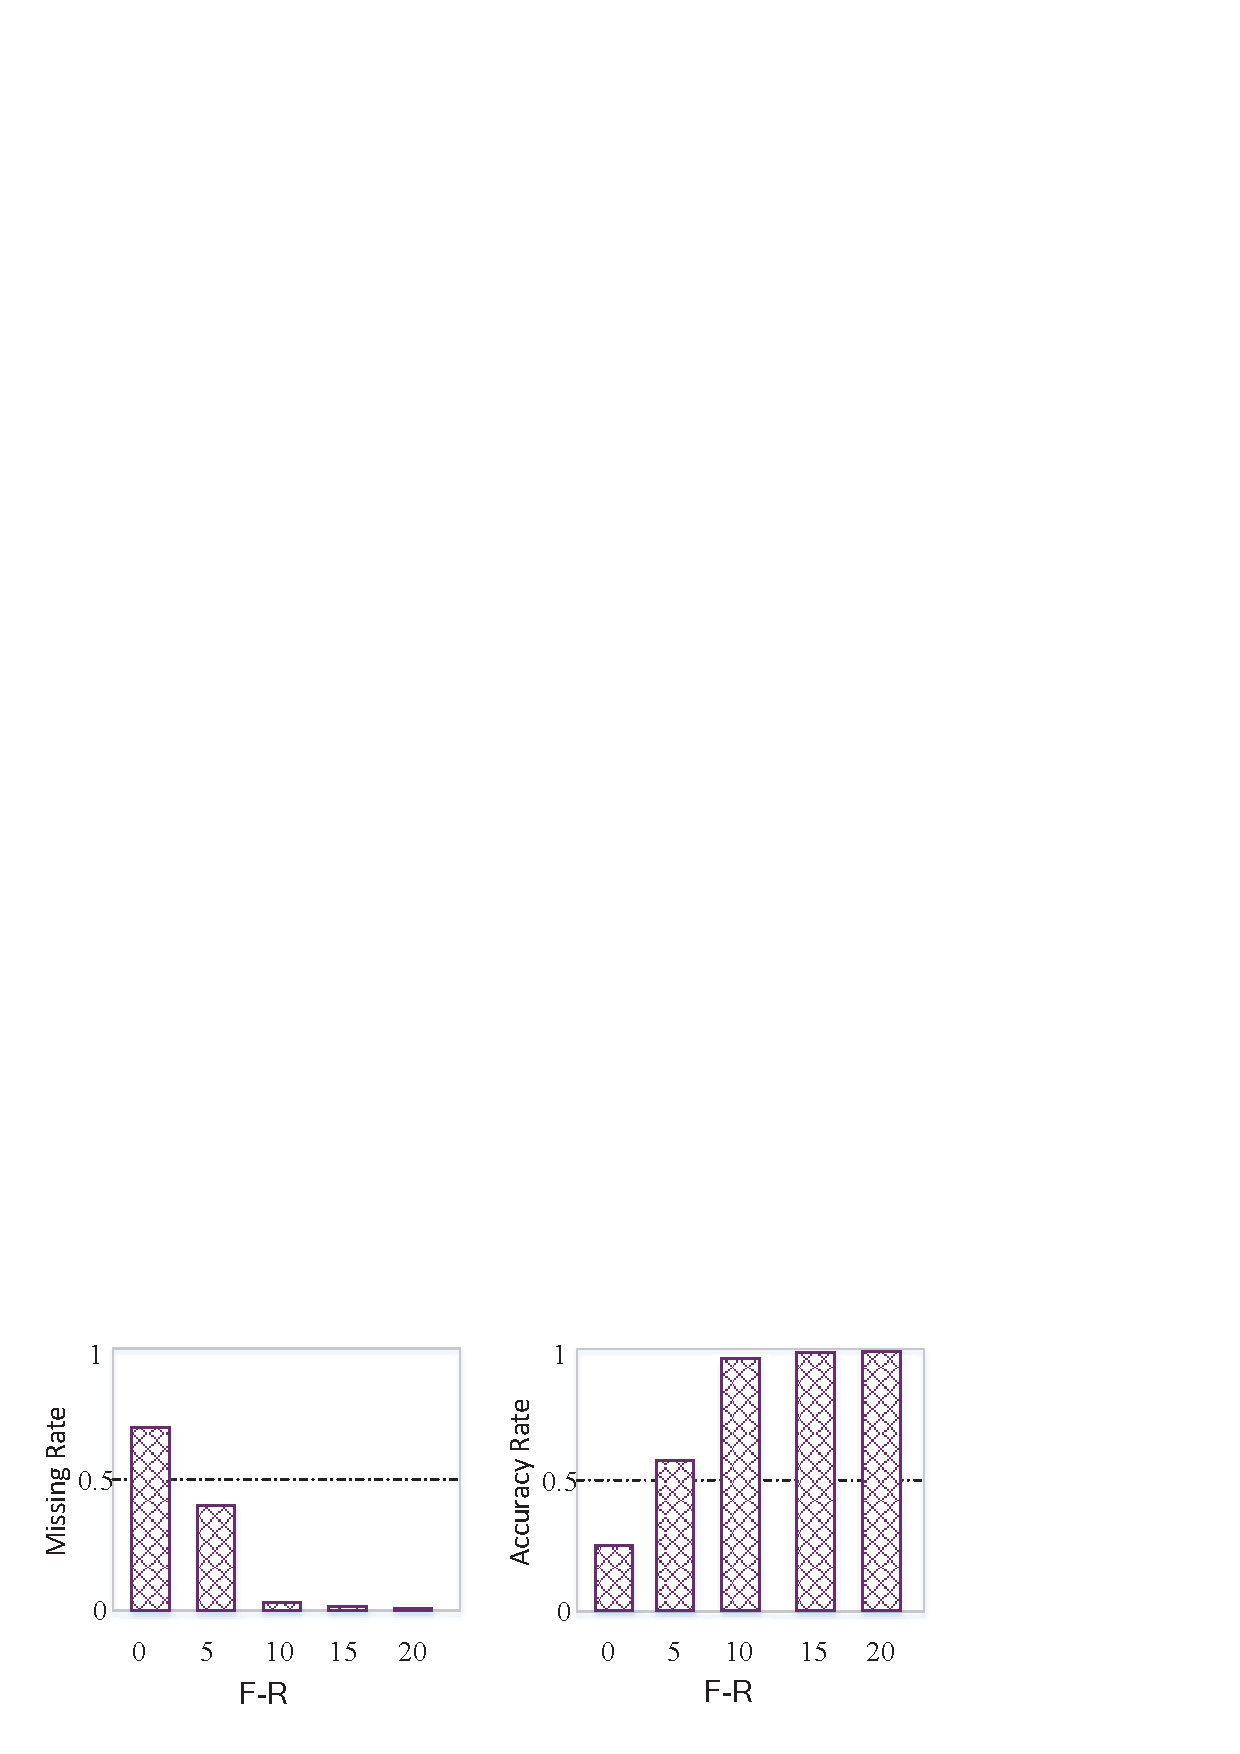
\includegraphics[width=1\textwidth]{figure/14.pdf}
\caption{Effect of distance on the detection results}
\end{figure}


\subsection{\secit Experiment and evaluation of multi position cooperative detection}

\textbf{Validation of variance increment method}

In this experiment, the window size is 120, and K is 4, then split the RSSI sequence using Variance increment method in the 6.2.1section. The result is shown as the Form 5. Dropping out the fragment whose length is shorter than 120, then we can get two effective RSSI sequence fragments (S\_1 and S\_10), the total length is 2598, the effective fragment length was 2605 in the original data sequence. So the accuracy is 99.7\%.

\begin{table}[h]
\centering
\caption{First time to split RSSI sequence}
\begin{tabular}{|c|c|c|c|c|} \hline
Flag&Range&Length&Range&Mean\\ \hline
S\_1 & 1-1422 & 1422 & [-52,-35] & -45.15 \\ \hline
S\_2 & 1366-1431 & 66 & [-44, -39] & -42.5\\ \hline
S\_3 & 1424-1502 & 79 & [-84, -38] & -50.04\\ \hline
S\_4 & 1489-1560 & 72 & [-100,-64] & -91.17\\ \hline
S\_5 & 1507-1569 & 63 & [-100,-87] & -95.95\\ \hline
S\_6 & 1552-1620 & 69 & [-100,-72] & -90.91\\ \hline
S\_7 & 1609-1718 & 110 & [-76, -38] & -56.54\\ \hline
S\_8 & 1660-1726 & 67 & [-75, -40] & -56.68\\ \hline
S\_9 & 1669-1731 & 63 & [-75, -40] & -59.95\\ \hline
S\_10 & 1861-2848 & 1168 & [-90, -56] & -66.37\\ \hline
\end{tabular}
\end{table}

\textbf{The validity of DTW algorithm}

To verify that the DTW algorithm could be used to choose the valid AP, we open the detecting software which could find all the AP and getting their RSSI. Then we let the detecting software move with the speed of 1.5m, staying at three different locations and staying at each place for 15 minutes. At the end, there are 28 APs being found, including 1 target AP and 27 candidate reference AP. For each of 27 candidate reference AP, we use DTW algorithm to calculate the distance of variance increment sequence between target AP and it. Finally, we are successful to find four suitable reference AP.

\textbf{The validity of localization algorithm}

In a room with 100 square meters, we collect a set of data per 4 square meters. So there are 25 sets of data. In detecting stage, we stayed at every position for 5 minutes, then moving to another position with the speed of 1.5m/s. For the four suitable reference AP found in previous section, there are three kinds of conditions, that is, the first 4 AP should be considered as the reference AP, and the first 3, the first 2, respectively calculate their Euclidean distance. When there is only one reference AP, the accuracy of location is 62\%. When there is two reference APs, the accuracy of location is 85\%. When there is three reference APs, the accuracy of location is 90\%.

\textbf{The validity of Multi position cooperative detection}

We play a role of an attack, simulating a fake AP in a notebook. And the experiment is done still in a room with 100 square meters, dividing it into 25 region. In each region, we collect data for every 30 minutes, and use the maximum mean of this region as the safety threshold. In detecting stage, we stayed at every position for 5 minutes, then moving to another position with the speed of 1.5m/s. Experiments were carried out for 200 times, 100 times is to open the fake AP, the other 100 times is to turn off the fake AP. When the fake AP is turned on, if there is any position detected by the fake AP, then the detection is successful, if all the positions are not detected by the fake AP, then the detection fails. Close the fake AP, if there is any position to detect the false AP, then the detection fails, if all the positions are not detected in the fake AP, then the detection successfully. When there is only one reference AP, the accuracy of location is 58\%. When there is two reference APs, the accuracy of location is 80\%. When there is three reference APs, the accuracy of location is 90\%.

\section{RELATED WORK}
At present, most Evil-Twin detection method work for the public WIFI environment. They are two key approaches in this domain. One is based on hardware feature, the other is flow feature.

The hardware feature testing method utilizes the characteristic that different network card chips and different drives possess different fingerprint features to set up a fingerprint feature library and decide whether the Fake AP is existed or not through matching fingerprint data in the fingerprint feature library during testing. Bratus et al.\cite{Bratus}  sends some SIMULATING frames which possess false formats but are not prohibited by a standard protocol. Although different network card chips or drives have different responses to various SIMULATING frames, the testing method is easy to be found by an intruder and the intruder can copy the feature. Franklin et al.\cite{2006} and Loh et al.\cite{fingerprinting} utilize the characteristic that different wireless network cards send different Probe Request frames with different periods during scanning to set up the fingerprint library. As the equipment only sends a small number of Probe Request during joining the network and the method can be valid when passive scanning is used, the expensive time overhead and the relatively bad real-time property are involved; Neumann et al. \cite{6258210} utilizes the arrival time of inter-frame space to identify the wireless equipment, but the characteristic can be faked by the intruder and the testing method based on the characteristic can be bypassed. The testing methods for the hardware fingerprint feature of the equipment above mentioned cut both ways: various fake AP can be tested effectively and the cost of faking the hardware feature of the intruder is relatively high; but the cost of building the hardware feature fingerprint library is high, the time for extracting the hardware fingerprint is long, the testing real-time property is worse, and the expansibility is bad.

According to the flow feature testing method, the network flow feature is different when the fake AP is existent or non-existent; so, whether Evil-Twin AP is existent or not can be tested. The method is excellent in extendibility, but also has some disadvantages. Beyah R et al. \cite{1378413,Wei} utilizes the arrival time space of each data packet to build a flow feature library; as the method is influenced by flow shaping greatly, the practical operation and the applicability is not good; Wei W et al. \cite{POR} proposes that the arrival time of the ACK data packet in a TCP protocol can be used to set up the flow feature library; as the arrival time is influenced by TCP, the testing efficiency is limited; Sheng B et al. \cite{6007016,Mano,682342} proposes that data round trip time can be used to test whether the fake AP is existent or not, but the data round trip time is influenced by the network type, the band width and the state of congestion at the same time.

Besides, Xu et al. \cite{5934960} puts forward the wireless fake AP attack in an in-vehicle network, meanwhile, gives the testing method based on RSSI. The method requires that all of the APs are equipped with GPS modules to report their own positions; a user judges whether the fake AP is existent or not through whether the measured RSSI is matched with the position or not. The method can effectively test the fake AP attack in the in-vehicle network, but is not suitable for indoor environment because the GPS signal is weakened, even shielded indoors.


\section{CONCLUSION}
In this paper, we propose a fake AP detection method based on RSSI in smart homes, whose essence is to detect whether the AP position is legal or not. Because AP's hardware features and traffic characteristics can be forged, but the location cannot be forged, so this method can effectively bypass the Evil-Twin Attack and being verify that can effectively reduce the detection delay and improve detection accuracy.

According to condition whether the detection position is fixed or not, there are two kinds of detection method based on RSSI is proposed. A single fixed position is simple in implementation and small amount of calculation, but the deployment location of detector will directly influence the detection results. If the deployment location is inappropriate, the detection rate is higher. Multi location collaborative detection need mobile phones involved in the detection, which is more complex, but can effectively solve the problem of missing some fake AP. It transforms Multi location collaborative detection into single fixed position detection by using the method of WIFI indoor location. At the end, the experimental results show that the method is feasible.


\section{ACKNOWLEDGMENTS}
This work was supported in part by the National Natural Science Foundation of China (No. 61373177, and No. 61572402), the Key Project of Chinese Ministry of Education (No. 211181), the International Cooperation Foundation of Shaanxi Province, China ((No. 2013KW01-02, No. 2015KW-003 and No. 2016KW-034), the China Postdoctoral Science Foundation (grant No. 2012M521797), the Research Project of Shaanxi Province Department of Education (No. 15JK1734), and the Research Project of NWU, China (No. 14NW28).





\bibliography{sigproc}
\end{document}

